\documentclass[conference]{IEEEtran}
\IEEEoverridecommandlockouts
% The preceding line is only needed to identify funding in the first footnote. If that is unneeded, please comment it out.
\usepackage{cite}
\usepackage{amsmath,amssymb,amsfonts}
\usepackage{algorithmic}
\usepackage{graphicx}
\usepackage{textcomp}
\usepackage{xcolor}
\usepackage{hyperref}
\usepackage{float}
\def\BibTeX{{\rm B\kern-.05em{\sc i\kern-.025em b}\kern-.08em
    T\kern-.1667em\lower.7ex\hbox{E}\kern-.125emX}}
\begin{document}

\title{Merkle Tree with Post-Quantum Secure Hash:
KangarooTwelve and Rescue\\
}

\author{\IEEEauthorblockN{ Henry Tran}
\IEEEauthorblockA{\textit{Electrical and Computer Engineering} \\
\textit{University of California, San Diego}\\
La Jolla, California \\
het002@ucsd.edu}
\and
\IEEEauthorblockN{Jeffrey Lee}
\IEEEauthorblockA{\textit{Electrical and Computer Engineering} \\
\textit{University of California, San Diego}\\
La Jolla, California \\
jsl019@ucsd.edu}
}

\maketitle

\begin{abstract}
We analyze and implement two different hashing functions from scratch, examining the implementation choices and optimizations made by the original authors. We further constructed a Merkle tree on top of each hash function, evaluating both CPU and GPU accelerated variants, and measure construction time, per node throughput, and cryptographic correctness across a range of tree sizes.

\end{abstract}

\begin{IEEEkeywords}
Cryptography, Keccak, SHA$-$3, KangarooTwelve, TurboSHAKE, Rescue Prime, Hashing, Merkle Tree, Data Structures, CUDA, Blockchain, Ledger Systems

\end{IEEEkeywords}

\section{Introduction}

The blockchain and distributed ledger systems requires highly secure and tamper proof ability of data. Making sure that data isn't getting tampered with makes sure that manipulation, unauthorized access, and theft can't occur and ensuring secure records transactions across a peer to peer network. This is where data structures like a Merkle Tree which can provide the security and  efficient, tamper evident proofs of data integrity. However the security of the Merkle Tree is dependent upon the underlying hashing functions. When selecting a hashing function is dependent upon those that are quantum resistant so that future attacks from future high powered quantum computers.

In our paper, we implemented both Rescue and KangarooTwelve hashing functions from scratch, validated the correctness against source solution, and implemented onto the Merkle tree, and validating the accuracy of the tree build and analyzing the performance difference from batching with a non batched CPU implementation and a batched GPU implementation of our hash functions.

\section{Background}

\subsection{KangarooTwelve}

KangarooTwelve is an extendable-output function (XOF) developed to enable high levels amount of security in its hashes. It was built as an optimization of SHA-3 KangarooTwelve was built on the Keccak-p$[1600, 12]$ permutation, which is a reduced round version of the full 24 round variant in the standard SHA-3 implementation. By doing this, throughput is 2x as a result of this. 

The structure of KangarooTwelve is that messages are broken down into 8192 byte chunks. The first chunk forms what is called the trunk and is processed directly. Each subsequent chunk is independently hashed via TurboSHAKE sponge with a dedicated domain separator to produce a 64 byte chaining value (CV). These CVs are appended to the trunk, which is then finalized with a count of how many CVs were produced and a terminator, before one final hash produces the output.

TurboSHAKE is the sponge construction underlying KangarooTwelve, in which its job is to take an arbitrary length input and produce an arbitrary length output, using the permutation as its core primitive. It does it by processing the input into 136 byte blocks (for 256 bit implementation) and then each block is XOR'd into the rate portion of the state, then the permutation is applied. Once we have gotten through all of the inputs, a final block is processed in which a separation byte is added and an ending byte before XORing once more. Overall this is part of the absorption phase. Afterwards we go through the squeeze phase, in which we would take our states and permute it one rate block at a time until we get to our final result. From here we are able to generate the desired hash we want.

\subsection{Rescue}
Rescue prime is a cryptographic hash function that is designed to be highly performant and efficient with Zero-Knowledge (ZK) proving systems (such as STARKs and SNARKs) and other verification protocols. Rescue-Prime achieves this efficient with ZK protocols by defining their hash function through finite field arithmetic operations, instead of traditiona bitwise operations done in standard hash functions like SHA-256 and SHA-3, to better align with the native mathematics in ZK proving systems.

Rescue prime is built on an arithmetic sponge construction which operates over a finite field $F_p$ where $p$ is a large prime number. Internally, the hash function keeps track of a "state" vector which is set to a specificed state width $m$ and can be broken down into two parts: the rate $r_p$ and capacity $c_p$ of the arithmetic sponge such that $m=r_p+c_p$. The sponge construction consists of two processes: absorbing and squeezing. The absorbing phase is when the hash function takes in the input data, pads it, and breaks it down into blocks of size $r_p$, these blocks are added to the state afterwhich the state undergoes the core permutation rounds. Next, the squeezing phase is when the hash values are extracted.

The core permutation is the Rescue-XLIX permutation which consists of six layers repeated over $N$ rounds.The layers are as follows: (1) Forward S-box: modular exponentiation across all exponents with exponent $\alpha$ (2) Linear Layer: Maximum Distance Separable (MDS) matrix multiplication (3) Constant Injection: adds pseudo-randomly generated constants to the state elements (4) Inverse S-box: modular exponentaition but this time with $\alpha^{-1}$ (5) Another Linear Layer (6) A final Constant Injection layer.

\subsection{Merkle Tree}

A Merkle Tree is a data structure that is commonly used in the blockchain, as it is an effective way to verify the integrity of data in distributed ledger systems. It allows for large sets of data to be summarized into a single hash, allowing for efficient and tamper-evident proof for validity.

The biggest advantage of Merkle Tree is that it is efficient in it's verification and validation. Because it only needs to prove that the transaction is part of the tree, as such it only needs to traverse upwards on the tree based on sibling hashes to the root, and if there is a match then validation is confirmed. It is fast and efficient and only really needing at most $O(log(N))$ time to properly varify and validate the transaction.

\section{Design Choices}

\subsection{KangarooTwelve}
Some of the design choices that went into KangarooTwelve are:

Reduced Rounds: Reducing the number of rounds needed to generate the permutations. This is as a result of known cryptanalytic attacks on Keccak require far fewer than 24 rounds to break, so 12 rounds provides an ample security margin while nearly doubling throughput.

Dividing into chunks: Having dividing the input message into chunks of 8192 bytes, it allows for the blocks to be ran in parallel. As such, dividing the states into equal sections allows for us to equally diving each section while being able to process each section in parallel as well.

\subsection{Rescue}
For our implementation of Rescue-Prime, we attempted to keep our design as close as possible to the specification of Rescue-Prime by the original authors. Many of these design choices were relevant to the choices of initialization parameters. For instance, our choice of MDS matrix was generated by building a Vandermonde matrix from $p$ and and the smallest primitive element of $F_p$. Our pseudo-random constants also strictly followed the specification by applying SHAKE256 to expand the ASCII string "Rescue-XLIX($p$, $m$, $c_p$, and $s$)" where each variable corresponds with the aforementioned initialization parameters and security level $s$. For our choice of $\alpha$ and consequently $\alpha^{-1}$, our selection follows that of the specification which computes $\alpha$ to be the smallest integer that is coprime with $p$. Lastly, the selection of the number of rounds of Rescue-XLIX permutations follows the computation to ensure resistance against the Groebner Basis Attack as recommended by the Rescue Prime authors.
As Rescue-Prime primarily consists of sequential permutations with layers of states that must be computed one-by-one, we focused opportutnites for parallelization in algorithmic operations such as the modular exponentiation applied to each element in the S-box layers of our Rescue-XLIX permutation rounds and the matrix multiplication with our MDS matrix.
\subsection{Merkle Tree}

Our implementation of Merkle Tree was designed with modularization in mind with our two hash functions. Our leaves and nodes are defined in a 2-dimensional CuPy/NumPy array. Enabling both hashfunctions to call node-by-node or batched level-by-level. By enabling batched hashing over our Merkle Tree's levels, we can leverage the most powerful accerlation on our GPU which is the ability to batch our hashing across many nodes at once on the GPU rather than node-by-nnode.

\section{Implementation}

Implementation can be found here:
\url{https://github.com/jxnlee/ucsd-ece268-project}

\subsection{KangarooTwelve}
When implementing KangarooTwelve, we followed the architecture laid out by the authors of the KangarooTwelve paper. 

On the permutation front, in the standard implementation (CPU), we unpacked the 200 byte state is unpacked into 25 64 bit unsigned integers stored as an array at the start of each invocation. And during each of the 12 rounds performed, we did the 5 step mappings. Where theta is performed and column parities are computed across all five columns and XOR'd into each lane with a one position rotation. And rho and pi are rotating bits in the lane and then permutes the lane position. Then chi is done, where it iterates over each of the five rows applying the non linear combination, before iota which will XOR the round constants in the lane. And for the CPU implementation each round is performed sequentially of each other.

When looking at the GPU implementation of this, we are virtually parallelizing the entirety of the keccak permutation portion of the code. Where because the states aren't directly related to each other, we can run in parallel to run theta, pi, rho, chi, and iota and have it generate all of our states before we run turboSHAKE. At the end, lanes are repacked to bytes at kernel exit. The kernel handles single hash calls in the standalone Kangaroo12 engine.

When going through turboSHAKE, we start with the absorb phase in which the input is processed in 136-byte rate blocks, each XOR'd byte by byte into the state before the permutation is applied. After all full blocks are absorbed, the remaining bytes are XOR'd in, then 0x80 is XOR'd into the last byte of the rate to mark end of padding. Afterwards, our result is squeezed by reading from the state one rate block at a time, and  applying the permutation again whenever more output is needed.


\subsection{Rescue}

When implementing Rescue-Prime, as previously mentioned, we strictly followed the implementation specified by the original authors algorithmically. We focused on implementing a form of the hash function that could seamless be initialized with the desired parameters and mode of computation (CPU vs GPU, batched vs sequential). With this in mind, we felt it most efficient to define a Rescue-Prime class type that could be used to initialize desired modes for our Rescue-Prime hash function. Pertaining to which device our hash function would run on, we ensured that our hash function could seamlessly swap between running on the CPU vs the GPU by defining the specific backend for our hash function to run on that would map the approparite array data structure to the desired device. This would not only ensure consistent functionality but would lead for intuitive and modular design. Furthermore, two types of hash functions were defined: one that hashes a single message, and another that would hash a list of messages, enabling us to leverage parallelism to run multiple hashes at once.

For GPU acceleration in our hash function itself, we focused on what could be parallelized, the moduler exponentiation mapped across state elements in each S-box layer of the Rescue-XLIX permutation, the matrix multiplication in the linear layer of the Rescue-XLIX permutation, and any other arithmetic operations. Much of this was handled in the CuPy backend of our implementation, but for modular exponentiation, we defined a custom kernel to map the arithmetic operation across each element in the state vector. We ensured that our GPU implementation maintained the state vector and any of its operations on the device to minimize high-latency message transfers between GPU and CPU.

\subsection{Merkle Tree}

For our implementation of Merkle Tree, we kept it as a modular frontend with a specified hash function backend that can be swapped out. With this in mind, we made sure to balance in our implementation a level of abstraction sufficient to make it modular while still maintaining optimal performance.

Since a significant amount of parallelization we can exploit comes from batching our hashing, we ensured that we could batch hashing wherever we could while still enabling sequential hashing for the CPU. We kept the implementation of our Merkle Tree to be straightforward to offload much of the parallelization and optimizations in the hash functions themselves so as to minimize complexity and ensure consistent results regardless of the hash that is being used. We kept as many operations as possible on the GPU for GPU enabled implementation, ensuring a kernel for each level of our Merkle Tree to optimize hash functions in the appropriate device, only maintaining sequential message passing as we go up the tree level-by-level. 

For Proof Generation and Verification, we ensured a high level implementation that could enable proof generation and verification regardless of what the hash function was. With our modular implementation, we only needed to worry about how we were interfacing with the elements and could apply our hash function accordingly through the interface. We are able to demonstrate later that our proof generation and verification is able to properly validate the integrity of the Merkle Tree.

\section{Results}

\subsection{KangarooTwelve}

When directly running Kangarootwelve against the benchmarks, we can see pretty consistent results throughout, where overall, having the parallelization of keccak permutations made significant contribution to performance. When analyzing the performance gains when making N amounts of hashes, each of a consistent size, we see the CPU implementation does struggle while the GPU implementation thrives. Where being able to parallelize the permutations allows for the hashing function to perform the steps needed faster and enables similar performance.

\begin{table}[h]
\centering
\footnotesize
\caption{Batched Hash Benchmark (8 KB messages)}
\begin{tabular}{|r|r|r|r|r|r|}
 \hline
 N & CPU (ms) & GPU (ms) & CPU & GPU  & Speedup \\
  &  &  & ($\mu$s/hash) & ($\mu$s/hash) &  \\
 \hline
  16           & 553.40        & 10.17          & 34587.74     & 635.80       & 54.40x \\
  256          & 8844.64       & 140.66         & 34549.38     & 549.46       & 62.88x\\ 
  4096         & 142207.89     & 2232.32        & 34718.72     & 545.00       & 63.70x\\
 \hline
\end{tabular}
\label{tab:exp1}
\end{table}

When we do also analyze the performance of hashing on larger message sizes, we can still see this general performance gain where being able to parallelize the lanes allows us to easily compute the absorption and squeezing effectively and efficiently. It also ensures that more time can be spent on turboSHAKE and the rest of the hashing function as it allows more overhead for portions that aren't parallelized to run in the amount of time needed.

\begin{table}[h]
\centering
\footnotesize
\caption{Variable Input Size Scaling (N = 1)}
\begin{tabular}{|l|r|r|r|r|r|}
 \hline
 Size & CPU (ms) & GPU (ms) & CPU & GPU & Speedup \\
 & &  & Throughput & Throughput & \\
 \hline
  16 B         & 0.547         & 0.169         & 0.03 MB/s     & 0.09 MB/s       & 3.24x\\
  8 KB         & 34.218        & 0.550         & 0.24 MB/s     & 14.91 MB/s       & 62.27x\\
  24 KB        & 102.414       & 1.295         & 0.24 MB/s     & 18.97 MB/s       & 79.07x\\
  48 KB        & 204.785       & 2.417         & 0.24 MB/s     & 20.33 MB/s       & 84.72x\\
  1 MB         & 4367.885      & 51.155        & 0.24 MB/s     & 20.50 MB/s       & 85.39x\\
  10 MB        & 43988.145     & 479.094       & 0.24 MB/s     & 21.89 MB/s       & 91.82x\\
 \hline
\end{tabular}
\label{tab:exp2}
\end{table}

\subsection{Rescue}

When directly running Rescue-Prime against the benchmarks, we can observe that the performance on the GPU drags behind the CPU significantly when it comes to hashing a large serial message sequentially (yielding 0.05x-0.06x speedup on average) as shown in the table below:

\begin{table}[h]
\centering
\footnotesize
\caption{Variable Input Size Scaling (Single Message)}
\begin{tabular}{|l|r|r|r|r|r|}
\hline
Size & CPU (ms) & GPU (ms) & CPU & GPU & Speedup \\
& & & Throughput & Throughput & \\
\hline
8 B   & 5.222    & 117.080   & 1.53 KB/s & 0.07 KB/s & 0.04x \\
512 B & 282.571  & 6002.964  & 1.81 KB/s & 0.09 KB/s & 0.05x \\
1 KB  & 563.163  & 11953.266 & 1.82 KB/s & 0.09 KB/s & 0.05x \\
4 KB  & 3124.725 & 47238.761 & 1.31 KB/s & 0.09 KB/s & 0.07x \\
8 KB  & 6001.716 & 94375.095 & 1.36 KB/s & 0.09 KB/s & 0.06x \\
\hline
\end{tabular}
\label{tab:exp2}
\end{table}

Regardless of the size of the message, the speedup from the GPU implementation is consistently worse than on the CPU. However, once we evaluate on batched messages, we see a drastic improvement in performance compared to the CPU. We can observe the results of running batched hashing based on the various size of messages shown in the table below:

\begin{table}[h]
\centering
\footnotesize
\caption{Batched Hash Benchmark (Fixed Message Size: 8 Bytes)}
\begin{tabular}{|r|r|r|r|r|r|}
\hline
N Messages & CPU Time & GPU Batch & CPU & GPU & Speedup \\
& (ms) & (ms) & us/hash & us/hash & \\
\hline
16   & 90.00    & 123.68  & 5625.20 & 7730.22 & 0.73x \\
256  & 1493.96  & 124.71  & 5835.78 & 487.14  & 11.98x \\
4096 & 23695.94 & 242.29  & 5785.14 & 59.15   & 97.80x \\
8192 & 47165.29 & 462.08  & 5757.48 & 56.41   & 102.07x \\
\hline
\end{tabular}
\label{tab:exp1}
\end{table}

This shows that for individual messages, parallelization with the GPU does not yield significant improvements but parallel batched hashes will be able to compensate with better performance on the collect batch of messages.

\subsection{Merkle Tree}

Before we run tree generation with Merkle on our hash functions, we first generated the results needed to verify the tree generation and verification. When we ran against SHA256, we were able to produce results that satisfies that the generation and verification is correct. Furthermore once, we ran against our two hash functions, we saw the same results as well.

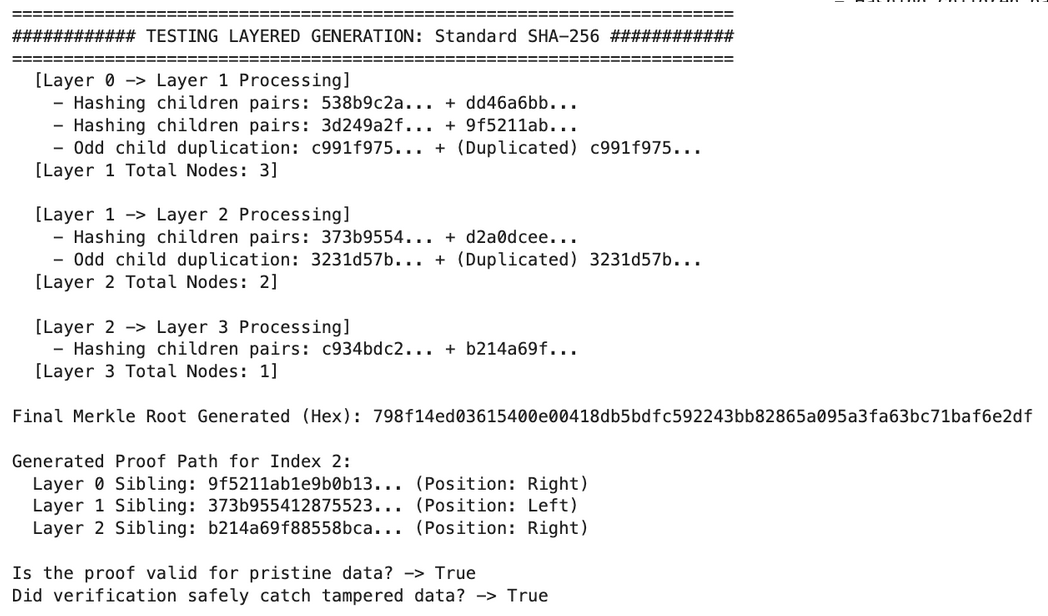
\includegraphics[scale=0.5]{Screenshot 2026-06-11 at 6.56.21 PM.png}

When we ran Merkle Tree, onto each of our hashing functions, we ended up seeing results that seem to be consistent with results we have seen and shown earlier.

In terms of KangarooTwelve, because of the heavily parallelization and amount of batching that can be seen, results portray higher level of performance on the tree generation on GPU. Where the building of the tree is significantly faster than the CPU counterpart. 

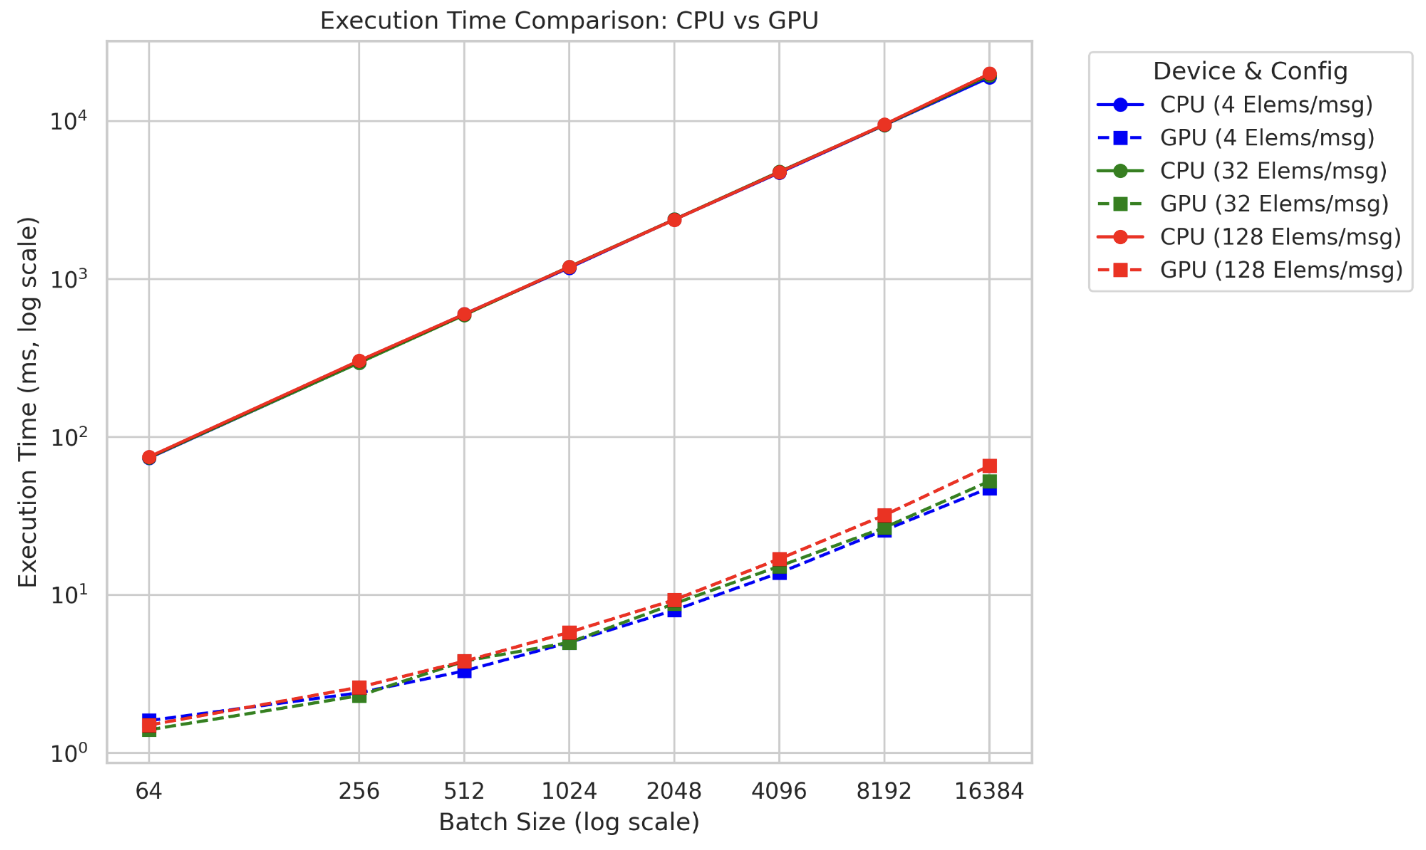
\includegraphics[scale = 0.25]{Screenshot 2026-06-11 at 6.19.15 PM.png}

Furthermore, because of the deeper level of parallelization, it enables higher levels of speedup, where the bigger and bigger the tree gets with larger batch sizes or message sizes, the better performing Kangaroo will get.

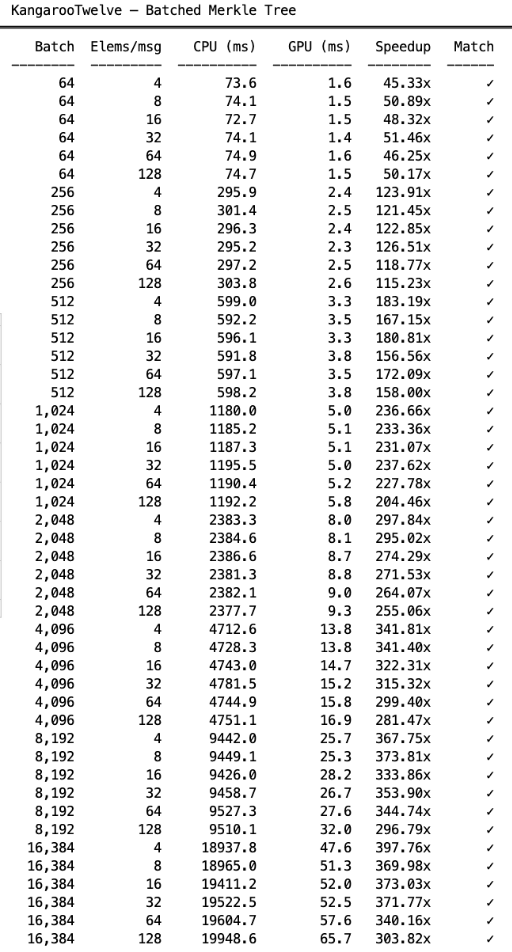
\includegraphics[scale=0.5]{Screenshot 2026-06-11 at 6.23.21 PM.png}

When we move over to Rescue-Prime, we end up seeing results that are consistent with what we thought would happen. 

When we look at the tree generation and the results produced from our Merkle Tree, we can see that the execution time of our Merkle Tree for our GPU implementation is getting out performed by the CPU on smaller sample sizes before eventually outperforming CPU by a significant margin once the batch size and messages sizes get large enough. And this is consistent with what we expect because of how much longer it takes for validation for Rescue-Prime to take. As such much of the performance gains will be from larger batches and larger message sizes as well.

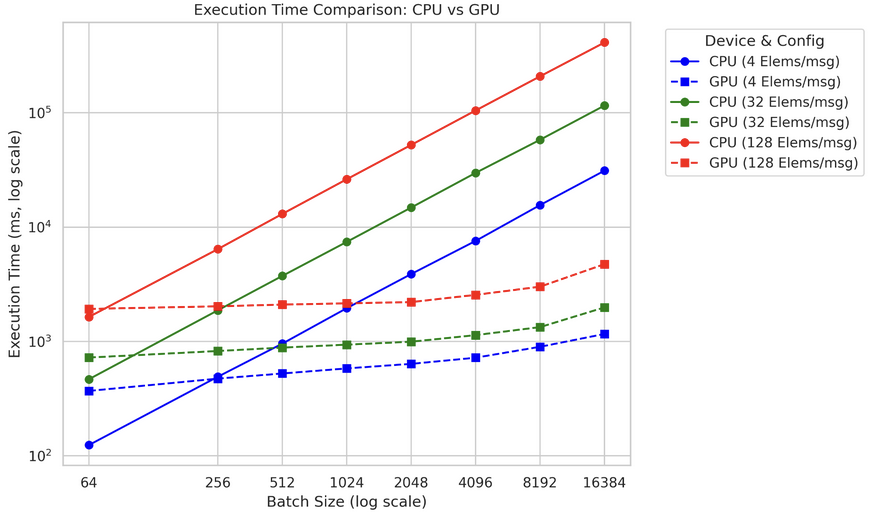
\includegraphics[scale=0.4]{Screenshot 2026-06-11 at 6.49.07 PM.png}

When we also analyze the build times it takes for each of our hash functions, it shows us directly what we have assumed. Where there is a high overhead the RescuePrime when using the GPU implementation. We can see that batching is important in the construction of our Merkle Tree. It shows how serial implementation has a large overhead in terms of performance and the construction of our tree.

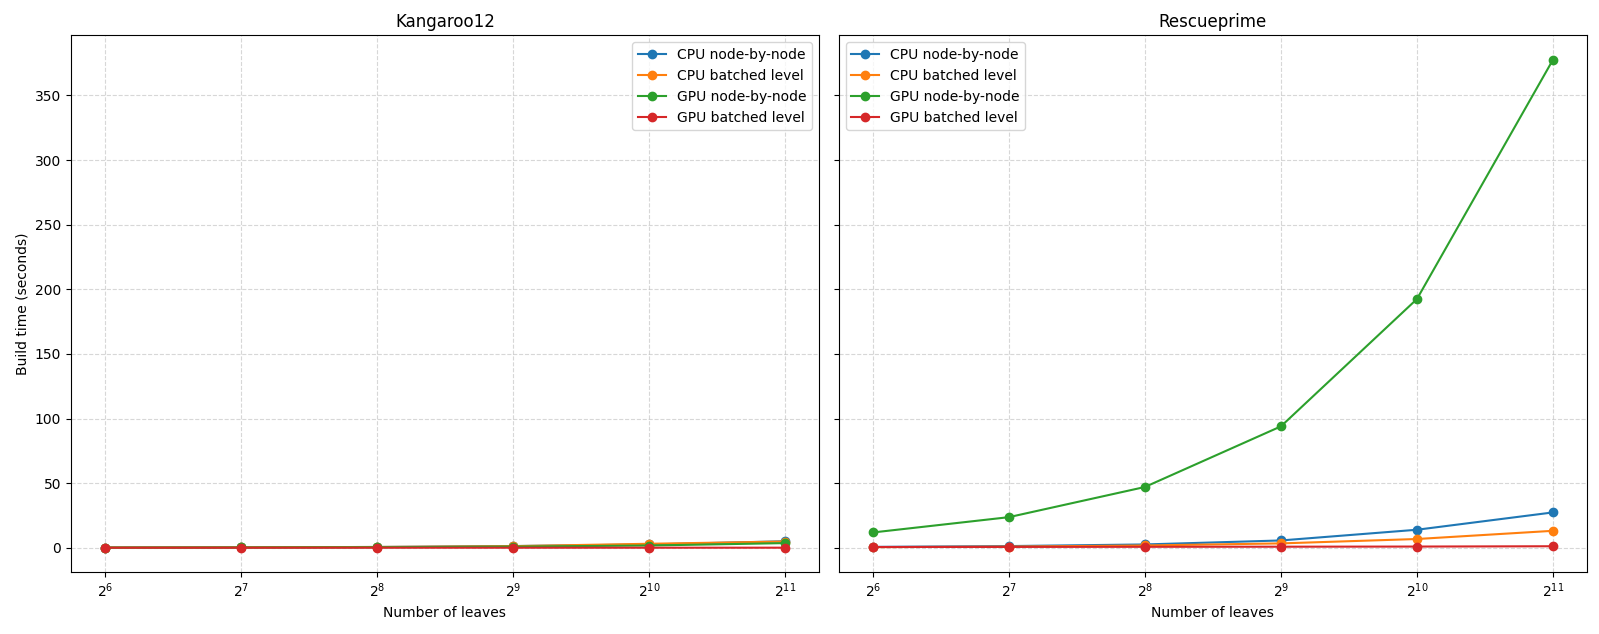
\includegraphics[scale = 0.15]{jfnewjkfnerwkjf.png}

\section{Conclusion}

To conclude, we were able to analyze the performance and correctness of using KangarooTwelve and Rescue-Prime with a Merkle Tree. We were able to understand the performance gains that KangarooTwelve gains from parallelization and how much we can parallelize it. And how the design choice that the authors made allowed for KangarooTwelve to be high performing yet highly secure. Furthermore, we understood the RescuePrime has a large overhead and such leads to problems with smaller inputs. Where to really maximize the performance gains with RescuePrime, we want to maximize the batches as otherwise a general CPU implementation will outperform it. Overall, some of the performance security tradeoffs feels minimal, where when we look at the tradeoffs for KangarooTwelve, we trade rounds in the permutations to get increased efficiency and speed. And when we truly analyze the tradeoffs that come from doing this, we lose out on a marginal amount of security.

As for Rescue-Prime, performance is a trade off that is made to improve performance in other areas. More specifically, it is highly optimized for efficient ZK proof verification while sacrificing performance on CPUs and GPUs. Nevertheless, no tradeoffs to the security of the hashing function is made and is specifically designed to fit needs where it is applied by enabling various levels of security through the computation and initialization of its parameters. While we specified and computed parameters for our implementation that would maximize security, we could surely select various parameters and optimize GPU kernels specific to given constants, in which case we may observe increased performance for reduced security. Nevertheless, with optimized security of our hash function, we were able to exploit parallelization wherever possible and obtain speedup with batched hashing.

With Merkle Tree we were able to demonstrate the strengths in batching our hash functions across levels and can subsequently observe how the efficiency in tree generation is improved. While proof generation and verification were not specifically benchmarked for performance, the implementation of Merkle Tree and application of our hash function enables highly efficient and consistent verification and validation of our hashing, ensuring the integrity of our data by detecting changes in the leaves of the Merkle Tree. Overrall, different hash functions have different tradeoffs in their implementation, especially with the requirements of our Merkle Tree, we can evaluate each aspect of how our hash functions perform. which hash function is implemented would ultimately depend on the needs of the user and application: whereas KangarooTwelve offers more efficient tree building, Rescue-Prime can offer efficiency if a system emphasizes ZK proof verification and is not bottlenecked by tree generation. 


\begin{thebibliography}{00}

\bibitem{turboshake_team}
Keccak Team, ``TurboSHAKE,'' 2023. [Online]. Available: \url{https://keccak.team/turboshake.html}

\bibitem{keccakp_team}
Keccak Team, ``Keccak-p permutations,'' 2023. [Online]. Available: \url{https://keccak.team/keccakp.html}

\bibitem{k12_team}
Keccak Team, ``KangarooTwelve,'' 2023. [Online]. Available: \url{https://keccak.team/kangarootwelve.html}

\bibitem{xkcp_k12}
XKCP, ``K12,'' GitHub repository, 2023. [Online]. Available: \url{https://github.com/XKCP/K12}

\bibitem{fips202}
National Institute of Standards and Technology, ``SHA-3 Standard: Permutation-Based Hash and Extendable-Output Functions,'' FIPS PUB 202, August 2015. [Online]. Available: \url{https://nvlpubs.nist.gov/nistpubs/fips/nist.fips.202.pdf}

\bibitem{rfc_k12}
G. Bertoni, J. Daemen, M. Peeters, G. Van Assche, R. Van Keer, and B. Viguier, ``KangarooTwelve and MarsupilamiFourteen,'' IETF Internet-Draft draft-irtf-cfrg-kangarootwelve-09, 2022. [Online]. Available: \url{https://www.ietf.org/archive/id/draft-irtf-cfrg-kangarootwelve-09.html}

\bibitem{merkle_wiki}
Wikipedia, ``Merkle tree,'' [Online]. Available: \url{https://en.wikipedia.org/wiki/Merkle_tree}

\bibitem{marvellous}
KULeuven-COSIC, ``Marvellous,'' GitHub repository, 2021. [Online]. Available: \url{https://github.com/KULeuven-COSIC/Marvellous}

\bibitem{rp_page}
Alan Szepieniec, Tomer Ashur, and Siemen Dhooghe, ``Rescue-Prime,'' [Online]. Available: \url{https://www.esat.kuleuven.be/cosic/sites/rescue/ }

\bibitem{symm_key_primitives}
Abdelrahaman Aly, Tomer Ashur, Eli Ben-Sasson, Siemen Dhooghe, Alan Szepieniec, ``Design of Symmetric-Key Primitives for Advanced Cryptographic Protocols'' Cryptology ePrint Archive, 2019. [Online]. Available: \url{https://eprint.iacr.org/2019/426.pdf}

\bibitem{rp_spec}
Alan Szepieniec, Tomer Ashur, and Siemen Dhooghe, ``Rescue-Prime: A Standard Specification (SoK)'' Cryptology ePrint Archive, 2020. [Online]. Available: \url{https://eprint.iacr.org/2020/1143.pdf}

\end{thebibliography}
\vspace{12pt}


\end{document}
